\chapter*{Introdução}
\addcontentsline{toc}{chapter}{Introdução}

Enquanto a aritmética lida com somas, diferenças, produtos e quocientes, o
cálculo lida com derivadas e integrais. A derivada e a integral podem
ser descritas em linguagem comum em termos de uma viagem de carro. O
painel de instrumentos de um automóvel possui um \emph{velocímetro}
com marcações em quilômetros por hora e uma agulha que indica a velocidade.
O painel de instrumentos também tem um \emph{odômetro} que totaliza a
distância viajada em quilômetros (a quilometragem).

\vspace{0.5\baselineskip}
\begin{minipage}{0.5\textwidth}
\begin{center}
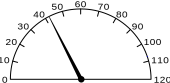
\includegraphics{figuras/introducao/velocimetro}\\
Velocímetro -- derivada da posição
\end{center}
\end{minipage}%
\begin{minipage}{0.5\textwidth}
\begin{center}
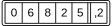
\includegraphics{figuras/introducao/odometro}\\
Odômetro -- integral da velocidade
\end{center}
\end{minipage}
\vspace{0.5\baselineskip}

Os valores indicados pelo velocímetro e pelo odômetro mudam com o tempo;
isto é, ambos são ``funções dependentes do tempo.'' A velocidade mostrada
no velocímetro é a taxa de variação, ou \emph{derivada}, da distância.
A velocidade é determinada tomando-se um intervalo de tempo muito
pequeno e calculando-se a razão entre a variação na distância e a
variação no tempo. A distância mostrada no odômetro é a
\emph{integral} da velocidade desde o instante inicial até o presente. 
A distância total é determinada pela adição das distâncias viajadas desde
o primeiro uso do carro até o presente.

O cálculo tem uma grande variedade de aplicações nas ciências naturais e
sociais. Algumas possibilidades estão ilustradas nos problemas.
Porém, é difícil prever futuras aplicações, portanto o próprio aluno
deve ser capaz de aplicar o cálculo a novas situações. Por esta razão, tão
importante quanto saber o que o cálculo pode fazer, é necessário aprender
por que ele funciona.
Para explicar por que o cálculo funciona, apresentaremos um grande número
de exemplos e desenvolveremos a teoria matemática com muito cuidado.

